%----------------------------------------------------------------------------------------
%	PACKAGES AND OTHER DOCUMENT CONFIGURATIONS
%----------------------------------------------------------------------------------------

\documentclass{beamer}

\usepackage[utf8]{inputenc}
\usepackage[T1]{fontenc}
\usetheme[numbering=fullbar]{focus}
% Add option [numbering=none] to disable the footer progress bar
% Add option [numbering=fullbar] to show the footer progress bar as always full with a slide count

%------------------------------------------------

\newcommand\blfootnote[1]{%
  \begingroup
  \renewcommand\thefootnote{}\footnote{#1}%
  \addtocounter{footnote}{-1}%
  \endgroup
}

%----------------------------------------------------------------------------------------
%	 TITLE SLIDE
%----------------------------------------------------------------------------------------

\title{Simulazione di blockchain:}
\subtitle{studio di alcuni casi di comportamento malevoli}

\author{\emph{Candidato:} Edoardo Rosa\\\emph{Relatore:} Gabriele D'Angelo}

\institute{\small{Scuola di Ingegneria e Architettura\\Corso di Laurea Magistrale in Ingegneria e Scienze Informatiche\\Università di Bologna}}

\date{\small{14-12-2018}}

%------------------------------------------------

\begin{document}

%------------------------------------------------

\begin{frame}
	\maketitle
\end{frame}

\begin{frame}
	\tableofcontents
\end{frame}

%----------------------------------------------------------------------------------------
%	 SECTION 1
%----------------------------------------------------------------------------------------

\section{Blockchain}
%------------------------------------------------

\begin{frame}{Blockchain - Bitcoin}
	Nel 2008 \textbf{Satoshi Nakatomo} pubblica\newline
    \textit{Bitcoin: A Peer-to-Peer Electronic Cash System}.\newline
    
    Un sistema di pagamento elettronico completamente \textbf{distribuito} e \textbf{decentralizzato} basato su \textbf{Blockchain} che risolve il problema dei generali Bizantini e del \textit{double spending}.
\end{frame}

\begin{frame}{Blockchain}
	\textit{Database} completamente \textbf{distribuito} che fa ampio uso di crittografia per eseguire applicazioni, salvare dati, trasferire asset digitali in maniera, \textbf{decentralizzata} e \textbf{append-only}.\newline
	\begin{figure}
    	\centering
        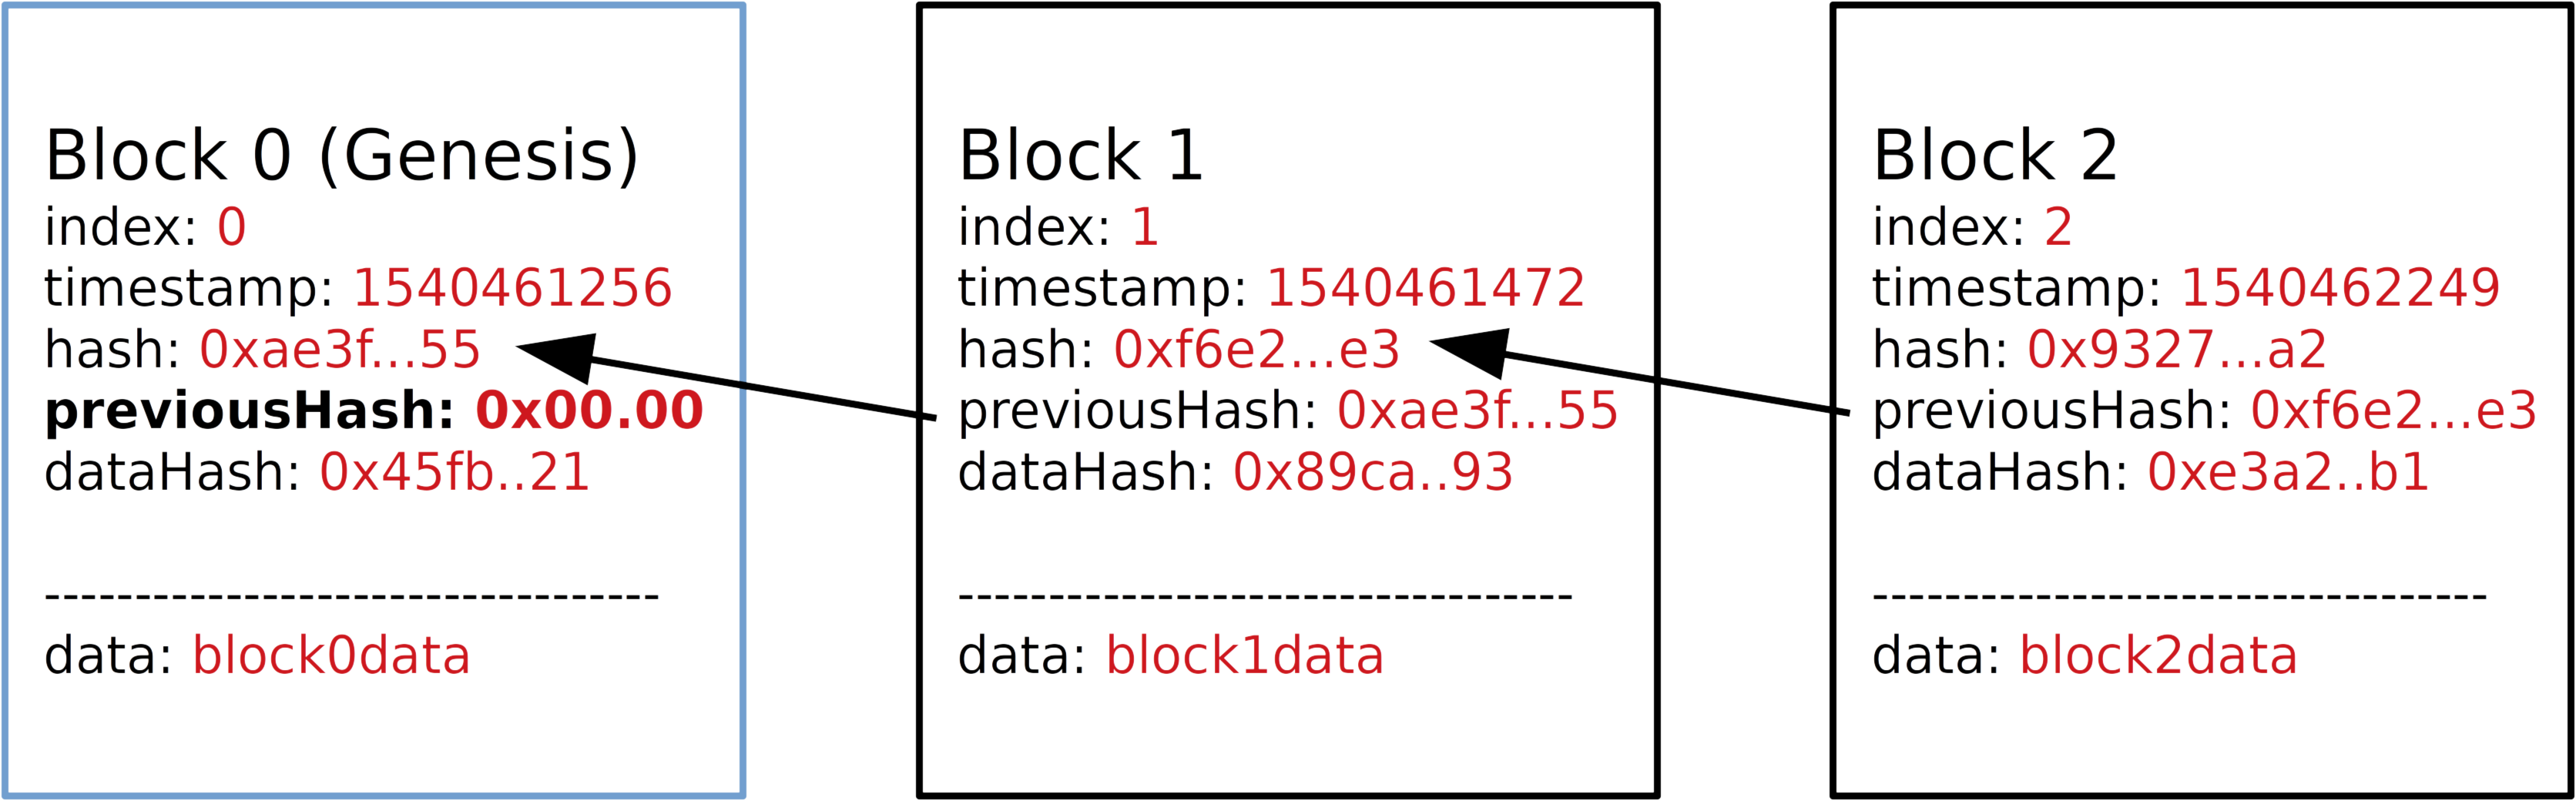
\includegraphics[width=\textwidth]{./images/blockchainbasic.png}
    \end{figure}
    	Tutte le transazioni sono raccolte all'interno del blocco e sono confermate solo quando sono aggiunte alla chain principale.
\end{frame}

%\begin{frame}{Blockchain - Transazioni}
%	Tutte le transazioni sono raccolte all'interno del blocco e sono confermate solo quando sono aggiunte alla chain principale.
%	\begin{figure}
%    	\centering
%        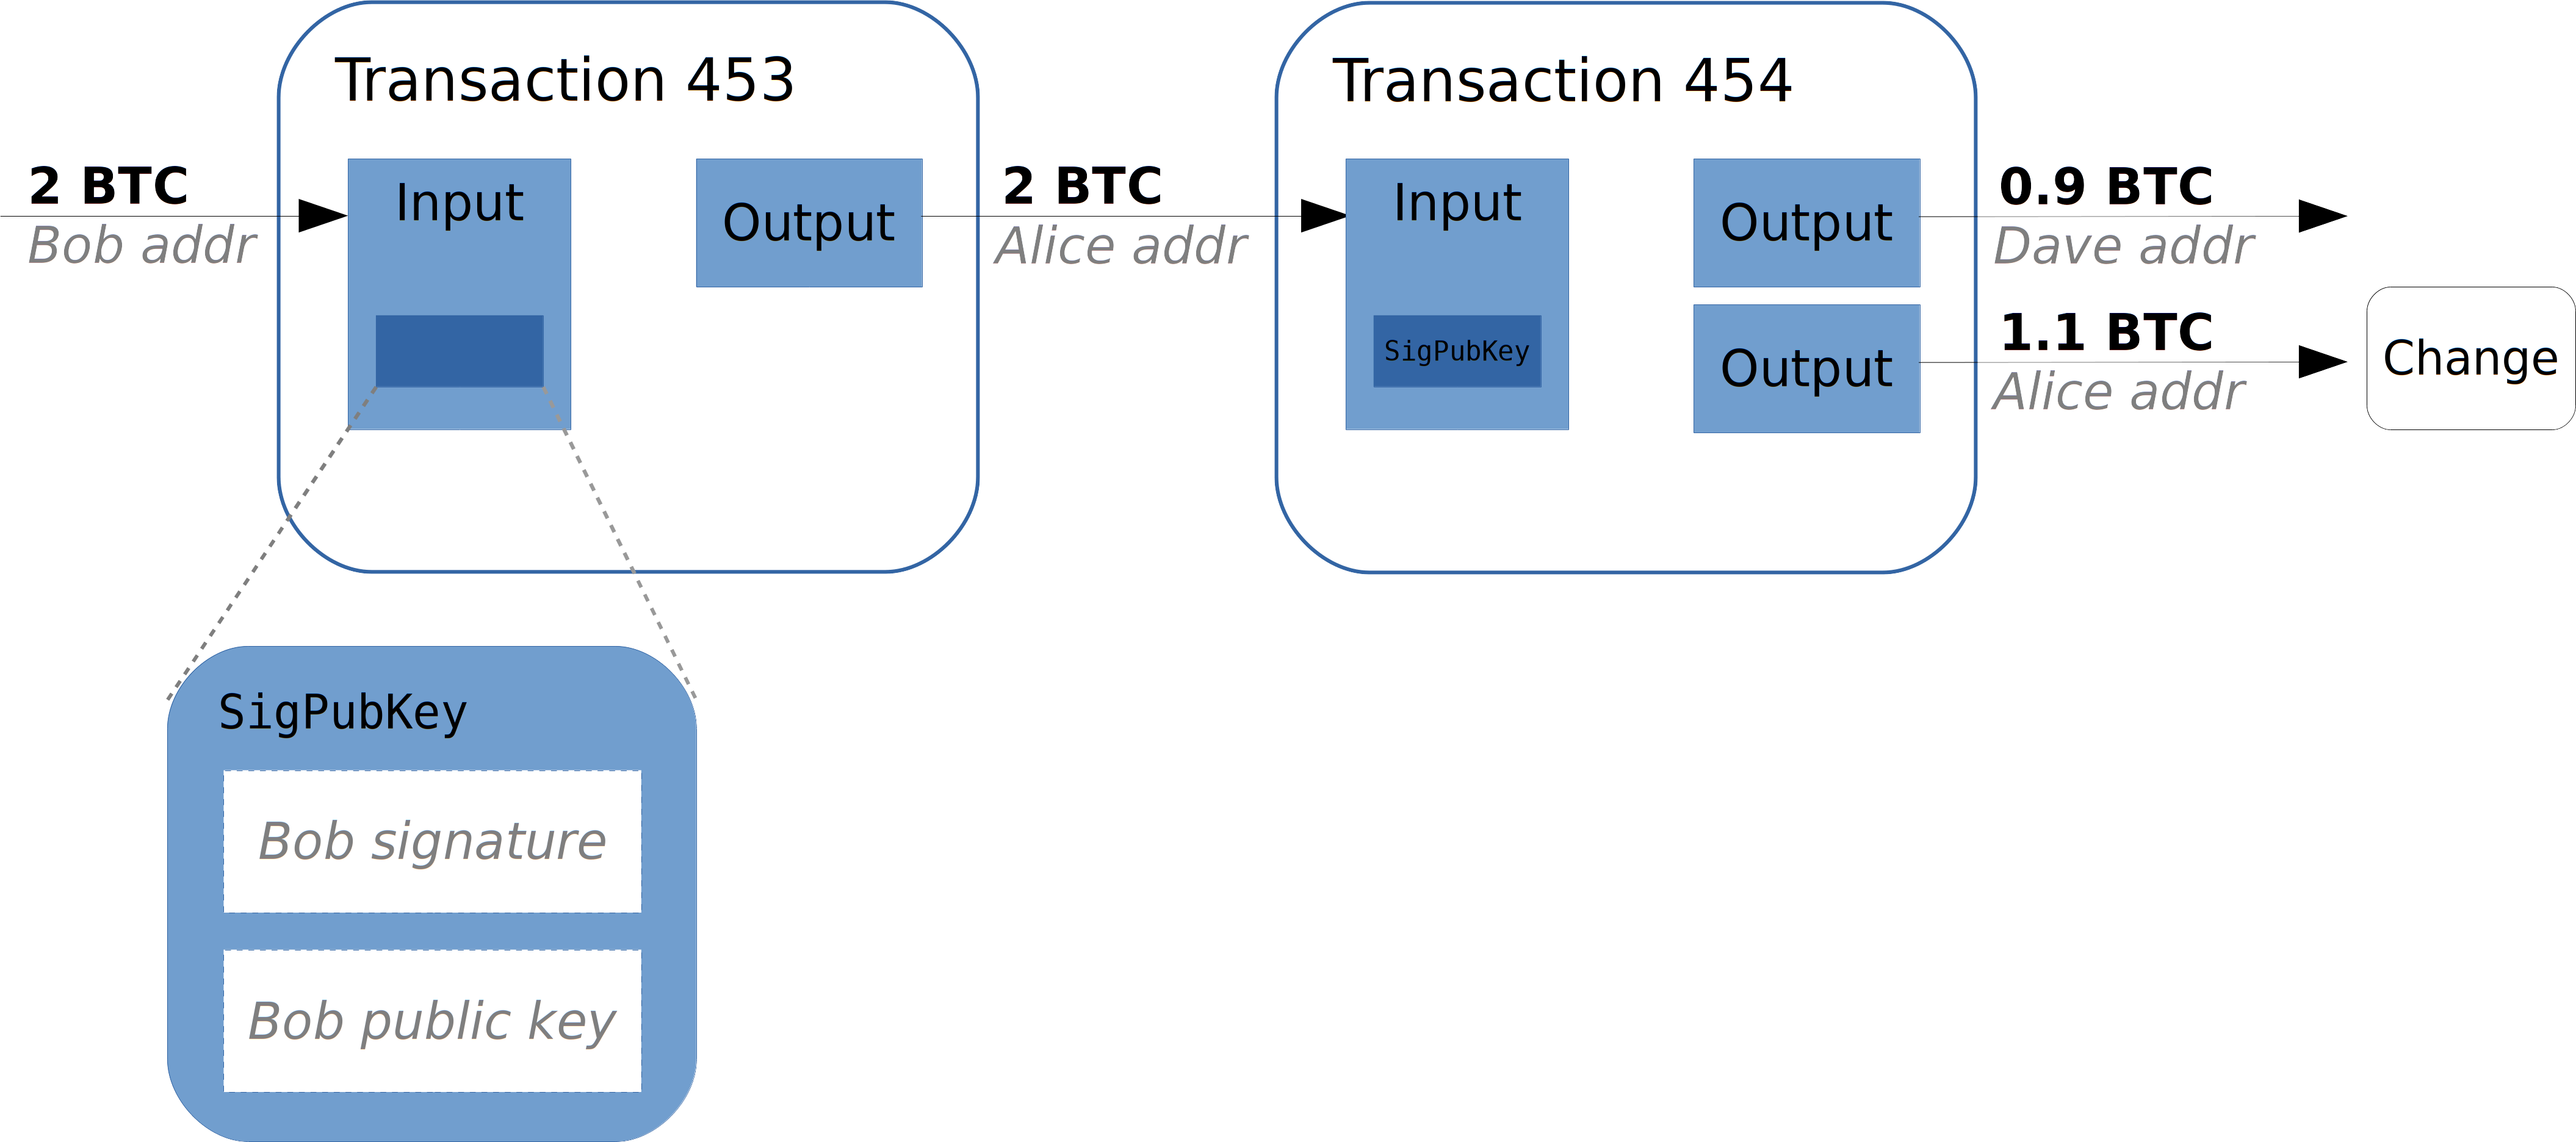
\includegraphics[width=\textwidth]{./images/tx-schema.png}
%    \end{figure}
%\end{frame}

\begin{frame}{Blockchain - Mining e \texttt{PoW}}
	Trovare un \textbf{nonce} $x$ tale per cui $h(k||x) < Y$.\newline
    
    Il protocollo formulato da Satoshi definisce che:
    \begin{itemize}
    	\item<1-> un blocco venga calcolato ogni 10 minuti
        \item<2-> \textit{hashcash}
        %\item<3-> i valori di $Y$ e $k$ variano ogni 2016 blocchi secondo la formula\newline
        \item<3->La probabilità $P$ di calcolare il \textit{nonce} corretto nel tempo $T$ è:
			\begin{equation}
    			P = \exp^{T/10}
   			\end{equation}
        %\begin{equation}
		%	D_{next} = (2016*10/T)* D_{prev}
        %\end{equation}
        %\begin{equation}
		%	Y = original\_target / D
		%\end{equation}
    \end{itemize}
\end{frame}

\begin{frame}{Blockchain - Rete}
	\begin{columns}
		\column{0.5\textwidth}
        	La \textbf{decentralizzazione} della rete Bitcoin è ottenuta utilizzando una rete \textit{peer-2-peer} che interagisce tramite \textbf{gossip}.\newline
            
            Ogni \textit{peer} della rete pubblica o riceve messaggi dai nodi vicini e mantiene aggiornata la propria blockchain locale.
		\column{0.5\textwidth}
			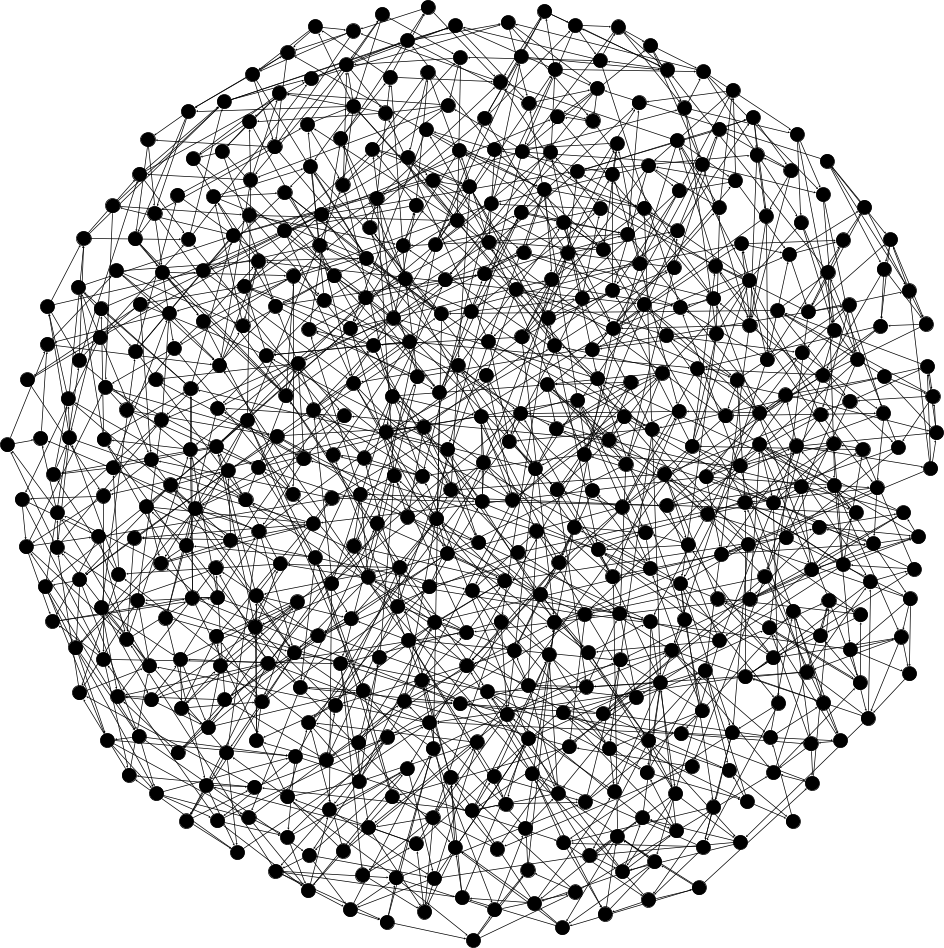
\includegraphics[width=\linewidth]{./images/network-500.png}
	\end{columns}
\end{frame}

%----------------------------------------------------------------------------------------
%	 SECTION 2
%----------------------------------------------------------------------------------------

\section[Implementazione di una blockchain su LUNES]{Implementazione~di~una\newline~blockchain su LUNES}

%------------------------------------------------

\begin{frame}{LUNES: Large Unstructured NEtwork Simulator}
	\begin{itemize}
		\item Distribuito
        \item Parallelo
        \item Basato su agenti
        \item Timestepped
        \item Reti \textit{peer-2-peer}
        \item Algoritmi di \textit{gossip} nativi
        \item Gestione automatica dello scambio dei messaggi (\texttt{ARTÍS})
        \item Load balancing (\texttt{GAIA})
       	\item Ottimizzazione dell'uso delle risorse
	\end{itemize}
\end{frame}

\begin{frame}{Messaggi}
	La simulazione prevede lo scambio di alcuni messaggi tra i nodi:
	\begin{block}{BlockMsg}
		Il \textit{nonce} corretto è stato trovato da un nodo e il blocco è stato pubblicato.
	\end{block}
	\pause % Automatically creates a new "page" split between the above and above + below
	\begin{block}{TransMsg}
		Un nodo ha creato una transazione che deve essere propagata nella rete affinché sia valida.
	\end{block}
	\pause % Automatically creates a new "page" split between the above and above + below
	\begin{block}{AskMsg}
		Un nodo richiede un particolare blocco della blockchain.
	\end{block}
\end{frame}

\begin{frame}{Ricezione di messaggi}
	\begin{figure}
		\centering
        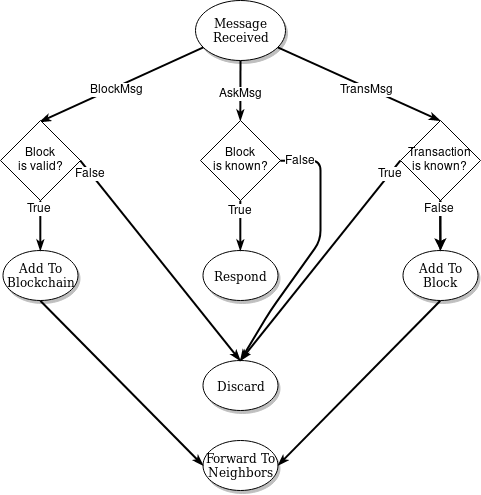
\includegraphics[width=0.65\linewidth]{./images/flow.png}
	\end{figure}
\end{frame}

%------------------------------------------------

\section{Attacchi}

\begin{frame}{DoS - Filtering}
	I nodi attaccanti agiscono come malevoli eliminando la fase di propagazione di messaggi creati dal nodo vittima.
    
    \begin{columns}
		\column{0.5\textwidth}
    		\begin{itemize}
    			\item 10000 nodi della rete
        		\item numero crescente di attaccanti
                \item 150 step di esecuzione
        		\item filtering di messaggi \textit{BlockMsg}
        		\item filtering di messaggi \textit{TransMsg}
        		\item filtering di messaggi \textit{AskMsg}
    		\end{itemize}
            
		\column{0.5\textwidth}
			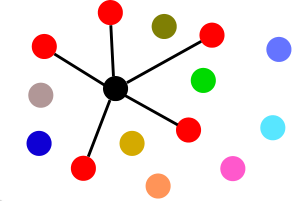
\includegraphics[width=\linewidth]{./images/sybil.png}
	\end{columns}
\end{frame}

\begin{frame}{DoS - Filtering - Risultati}
	\begin{figure}
		\centering
        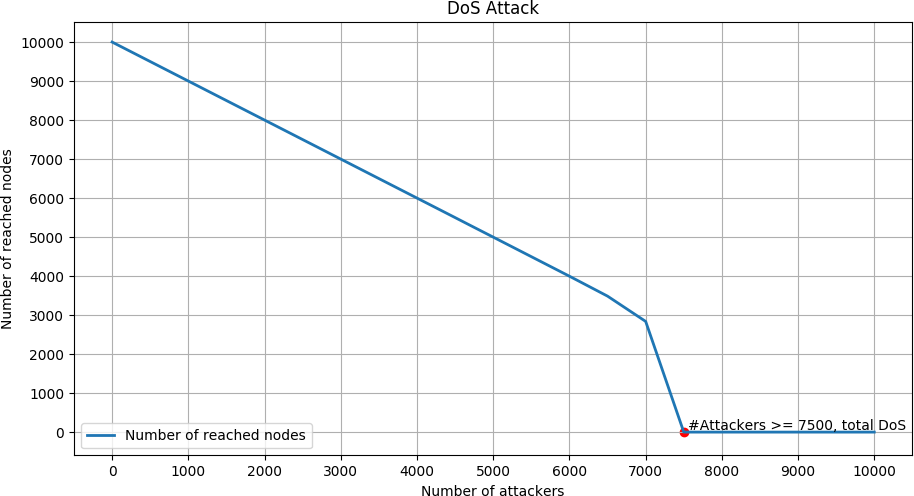
\includegraphics[width=\linewidth]{./images/attackDOS.png}
	\end{figure}
\end{frame}

\begin{frame}{DoS - Filtering - Risultati}
	\begin{figure}
		\centering
        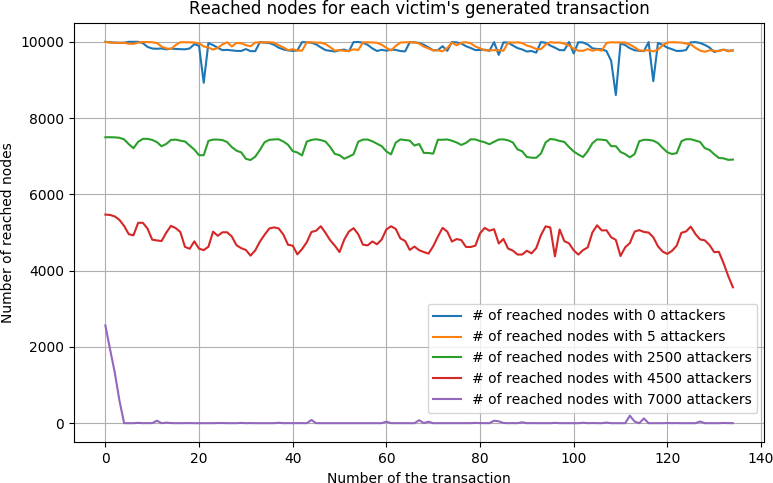
\includegraphics[width=\linewidth]{./images/DOS-mix.png}
	\end{figure}
\end{frame}


\begin{frame}{51\% e Double Spending}
    Per un \textit{miner} $m$ con una frazione $h$ dell'\textit{hashrate} totale $H$, l'equazione diventa:
   	\begin{equation}
    	P_{m} = \frac{(h*H/100) * T}{2^{32} * D}
    \end{equation}
    All'aumentare della potenza di calcolo aumenta la probabilità di \textit{mining} di un blocco in un tempo $T$.
\end{frame}

\begin{frame}{51\% e Double Spending}
	\begin{figure}
		\centering
        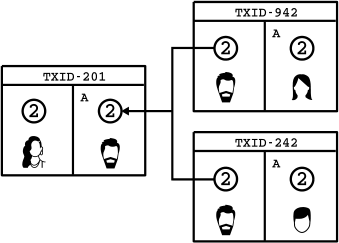
\includegraphics[width=0.6\linewidth]{./images/double_spending.png}
	\end{figure}
    Con la transazione numero \emph{942} Bob cede dei Bitcoin ad Alice tramite la UTXO \emph{201} ma al tempo stesso utilizza lo stesso output per una transazione verso Carol (\emph{242}).
\end{frame}

\begin{frame}{51\% e Double Spending}
	Il nodo attaccante controlla l'evoluzione della blockchain in quanto possiede la maggioranza della potenza di calcolo.
    
    \begin{itemize}
    	\item 10000 nodi della rete
        \item hashrate dell'attaccante crescente
        \item 5000 step di esecuzione
        \item 15 miner ``onesti''
        \item nessun tentativo di \textit{double spending}
    \end{itemize}
\end{frame}

%\begin{frame}{51\% e Double Spending - Risultati}
%    \begin{columns}
%		\column{0.5\textwidth}
%			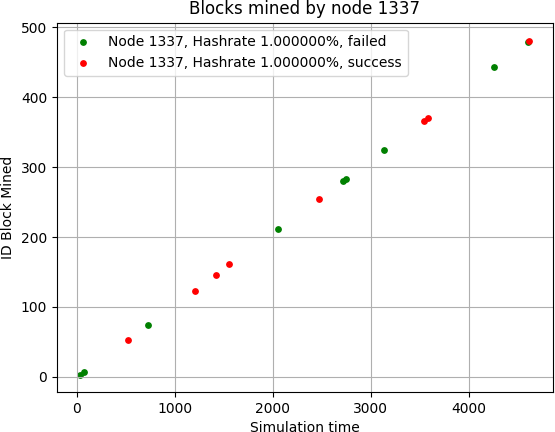
\includegraphics[width=\linewidth]{./images/1337-test-51-1.png}
%            
%		\column{0.5\textwidth}
%			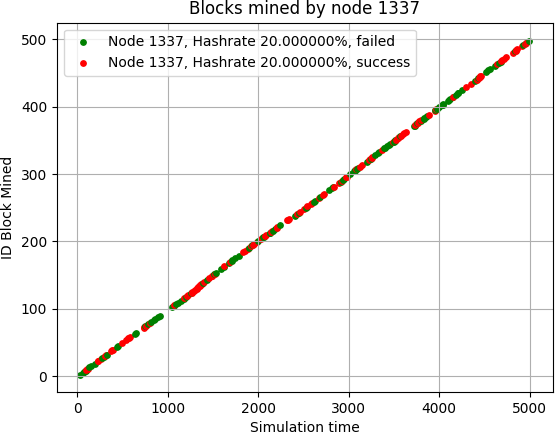
\includegraphics[width=\linewidth]{./images/1337-test-51-20.png}
%	\end{columns}
%\end{frame} 

\begin{frame}{51\% e Double Spending - Risultati}
	\begin{figure}
		\centering
        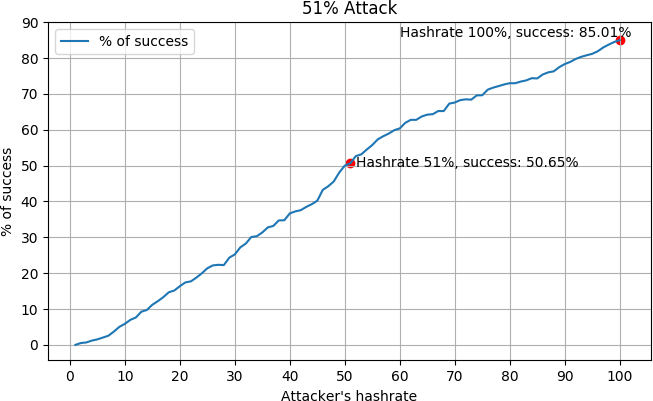
\includegraphics[width=0.9\linewidth]{./images/51-v3.png}
	\end{figure}
\end{frame}

\begin{frame}{Selfish Mining}
	L'attaccante applica la strategia di \textit{selfish mining} al fine di ottenere maggiori ricavi dall'attività di \textit{mining} generando delle \textit{race condition} tra i blocchi propagati in rete.
    \begin{columns}
		\column{0.5\textwidth}
    		\begin{enumerate}
    			\item l'attaccante trova un nuovo blocco ma non lo propaga
                \item se l'attaccante riceve un blocco dai nodi vicini propaga il blocco trovato un precedenza
                \item se l'attaccante trova un secondo blocco li propaga entrambi e l'attacco ha successo
    		\end{enumerate}
            
		\column{0.5\textwidth}
			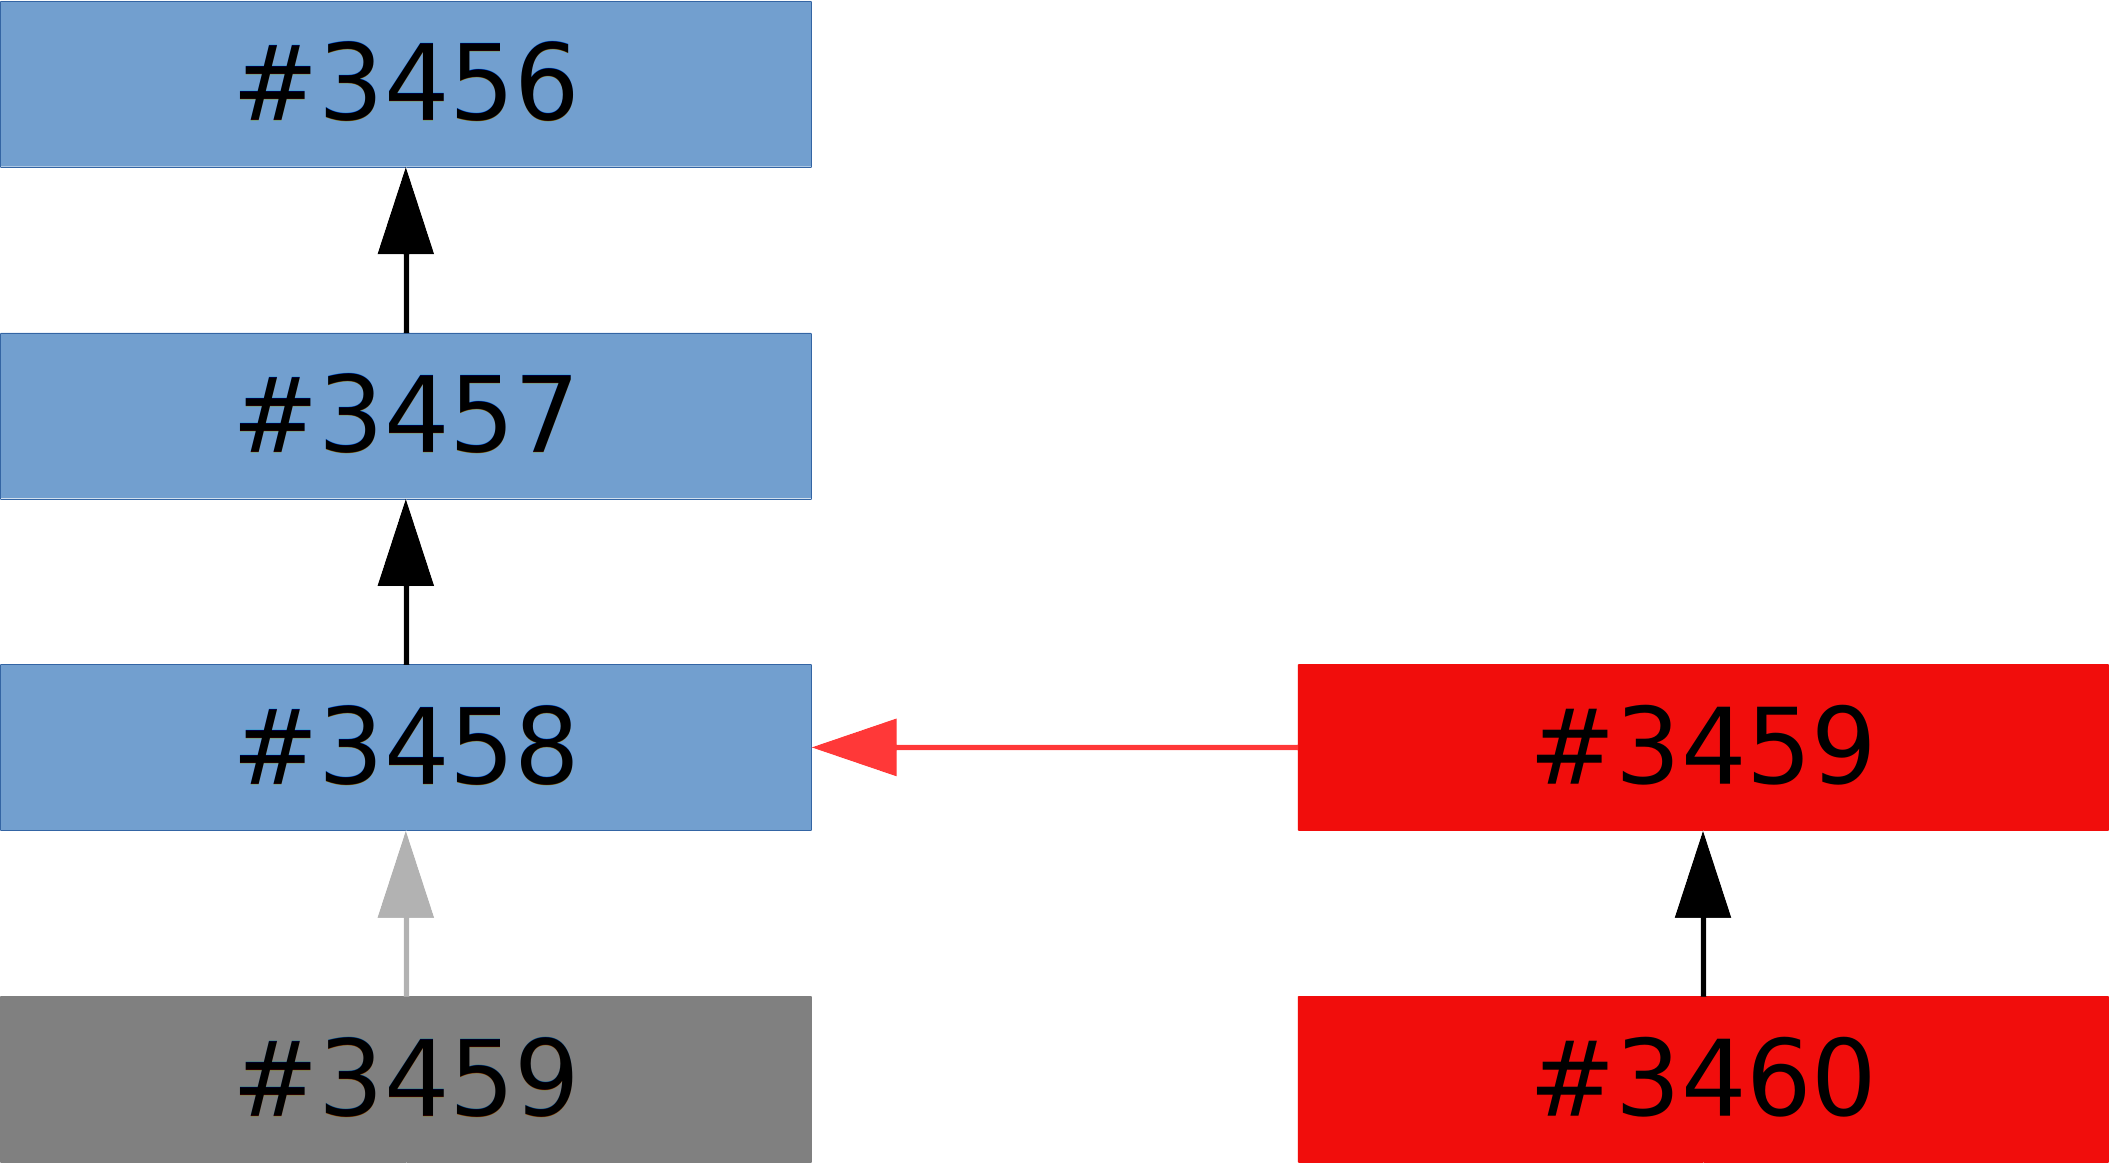
\includegraphics[width=\linewidth]{./images/selfish.png}
	\end{columns}
\end{frame}

\begin{frame}{Selfish Mining}
	\begin{itemize}
    	\item 10000 nodi della rete
        \item hashrate dell'attaccante crescente
        \item 5000 step di esecuzione
        \item 15 miner ``onesti''
        \item 1 miner con strategia di \textit{selfish mining}
    \end{itemize}
\end{frame}

\begin{frame}{Selfish Mining - Risultati}
	\begin{figure}
		\centering
        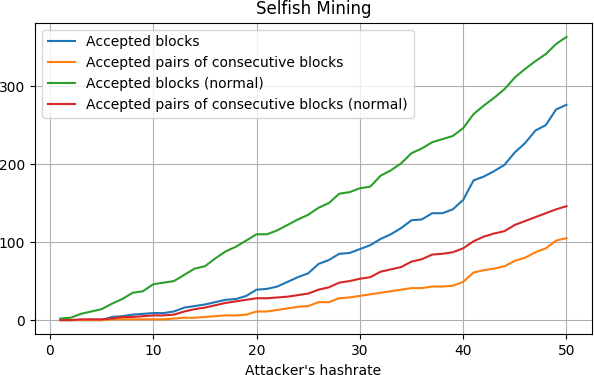
\includegraphics[width=0.9\linewidth]{./images/selfishtest.png}
	\end{figure}
\end{frame}


\section{Conclusioni}

\begin{frame}[plain]    
   	I risultati ottenuti rispecchiano i dati proposti dagli studi teorici e sono importanti al fine di identificare delle soglie limite per cui un'eventuale presenza di un attore malevolo può mettere in difficoltà l'intera rete Bitcoin.
    \vfill    
    Tramite \textit{LUNES} è stato possibile creare e testare alcuni scenari di comportamenti malevoli fino ad ora solo teorizzati garantendo una base per ulteriori integrazioni ed applicazioni.
\end{frame}

\begin{frame}[focus]
	Grazie per l'attenzione
\end{frame}

%----------------------------------------------------------------------------------------
%	 CLOSING/SUPPLEMENTARY SLIDES
%----------------------------------------------------------------------------------------

\appendix

%------------------------------------------------
% Slides di backup in caso di domande

\section{Appendice}

\begin{frame}{Costo 51\%}
	Con gli attuali valori di hashrate il costo per ottenere il 51\% di potenza per un'ora tramite cloud computing è di \textbf{14~682~645\$}.\vfill    
    In un'ora vengono pubblicati circa $6$ blocchi per un possibile reward totale di $75$ BTC, ovvero \textbf{476~175\$}, che potrebbe essere utilizzato per ammortizzare il costo iniziale.
	\vfill
	Per criptomonete minori invece il \textit{threat} è concreto e sono diversi gli attacchi avvenuti con successo.
\end{frame}

\begin{frame}{Blockchain - Problema dei Generali Bizantini}
	Raggiungere il \textbf{consenso} in situazioni in cui è possibile la presenza di errori.
	\begin{figure}
    	\centering
        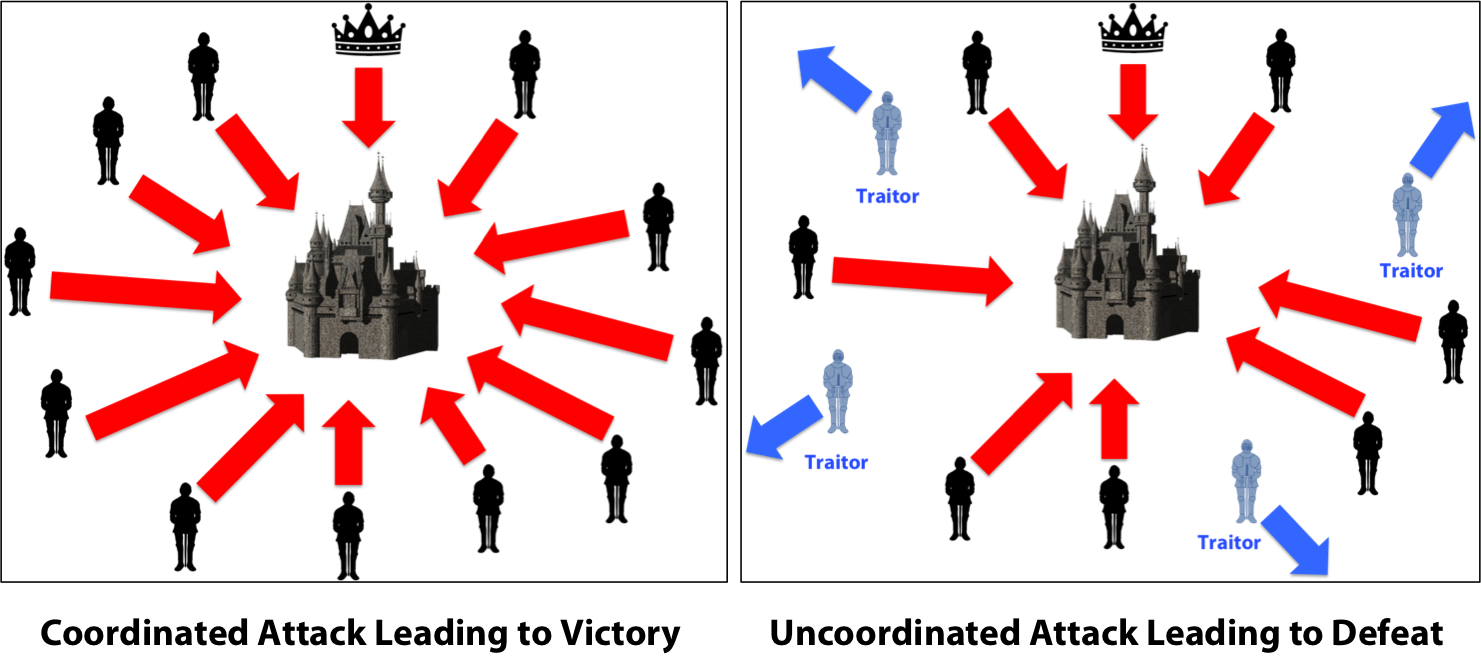
\includegraphics[width=\textwidth]{./images/byzantine.png}
    \end{figure}
\end{frame}

\begin{frame}{Diffusione Bitcoin}
	\begin{figure}
		\centering
        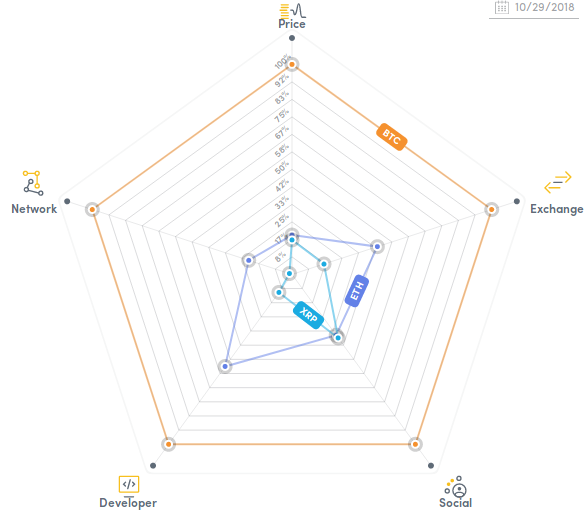
\includegraphics[width=0.8\linewidth]{./images/crypto_economics.png}
	\end{figure}
\end{frame}

\begin{frame}{Identità Sathosi Nakamoto}
	\begin{itemize}
        \item appartenente al mondo \textit{cypherpunk}
        \item sicurezza personale
        \item prevenzione legale
        \item notevole ammontare di BTC
        \item wallet: \emph{1A1zP1eP5QGefi2DMPTfTL5SLmv7DivfNa}
    \end{itemize}
\end{frame}

%----------------------------------------------------------------------------------------

\end{document}
